
\section{Results}
\label{sec:results}

In Figures \ref{fig:3dplot1} to \ref{fig:3dplot4}, we demonstrate network scalability as a function of QoI requirements for different traffic properties in a mesh setting.


%\begin{figure}
%\centering
%  \subfigure[Average Coverage vs. Energy Budget]{
%    \includegraphics[scale=0.35]{figures/mds_mobile/vary_power_budget/initBattery_7000/IR_3_nodes_5/send_size_2200_cov_size_135/perc_cov_vs_pow_budg.pdf}
%    \label{fig:avg_cov_vary_pow_budg}
%    }
%    \subfigure[Average Energy vs. Energy Budget]{
%    \includegraphics[scale=0.35]{figures/mds_mobile/vary_power_budget/initBattery_7000/IR_3_nodes_5/send_size_2200_cov_size_135/avg_pow_vs_pow_budg.pdf}
%    \label{fig:avg_pow_vary_pow_budg}
%    }
%\caption{Performance for Varying Energy Budget.}
%\label{fig:vary_pow_budg_all_algs}
%\end{figure}

\begin{figure}
\centering
    
    \subfigure[Unicast Traffic]{
        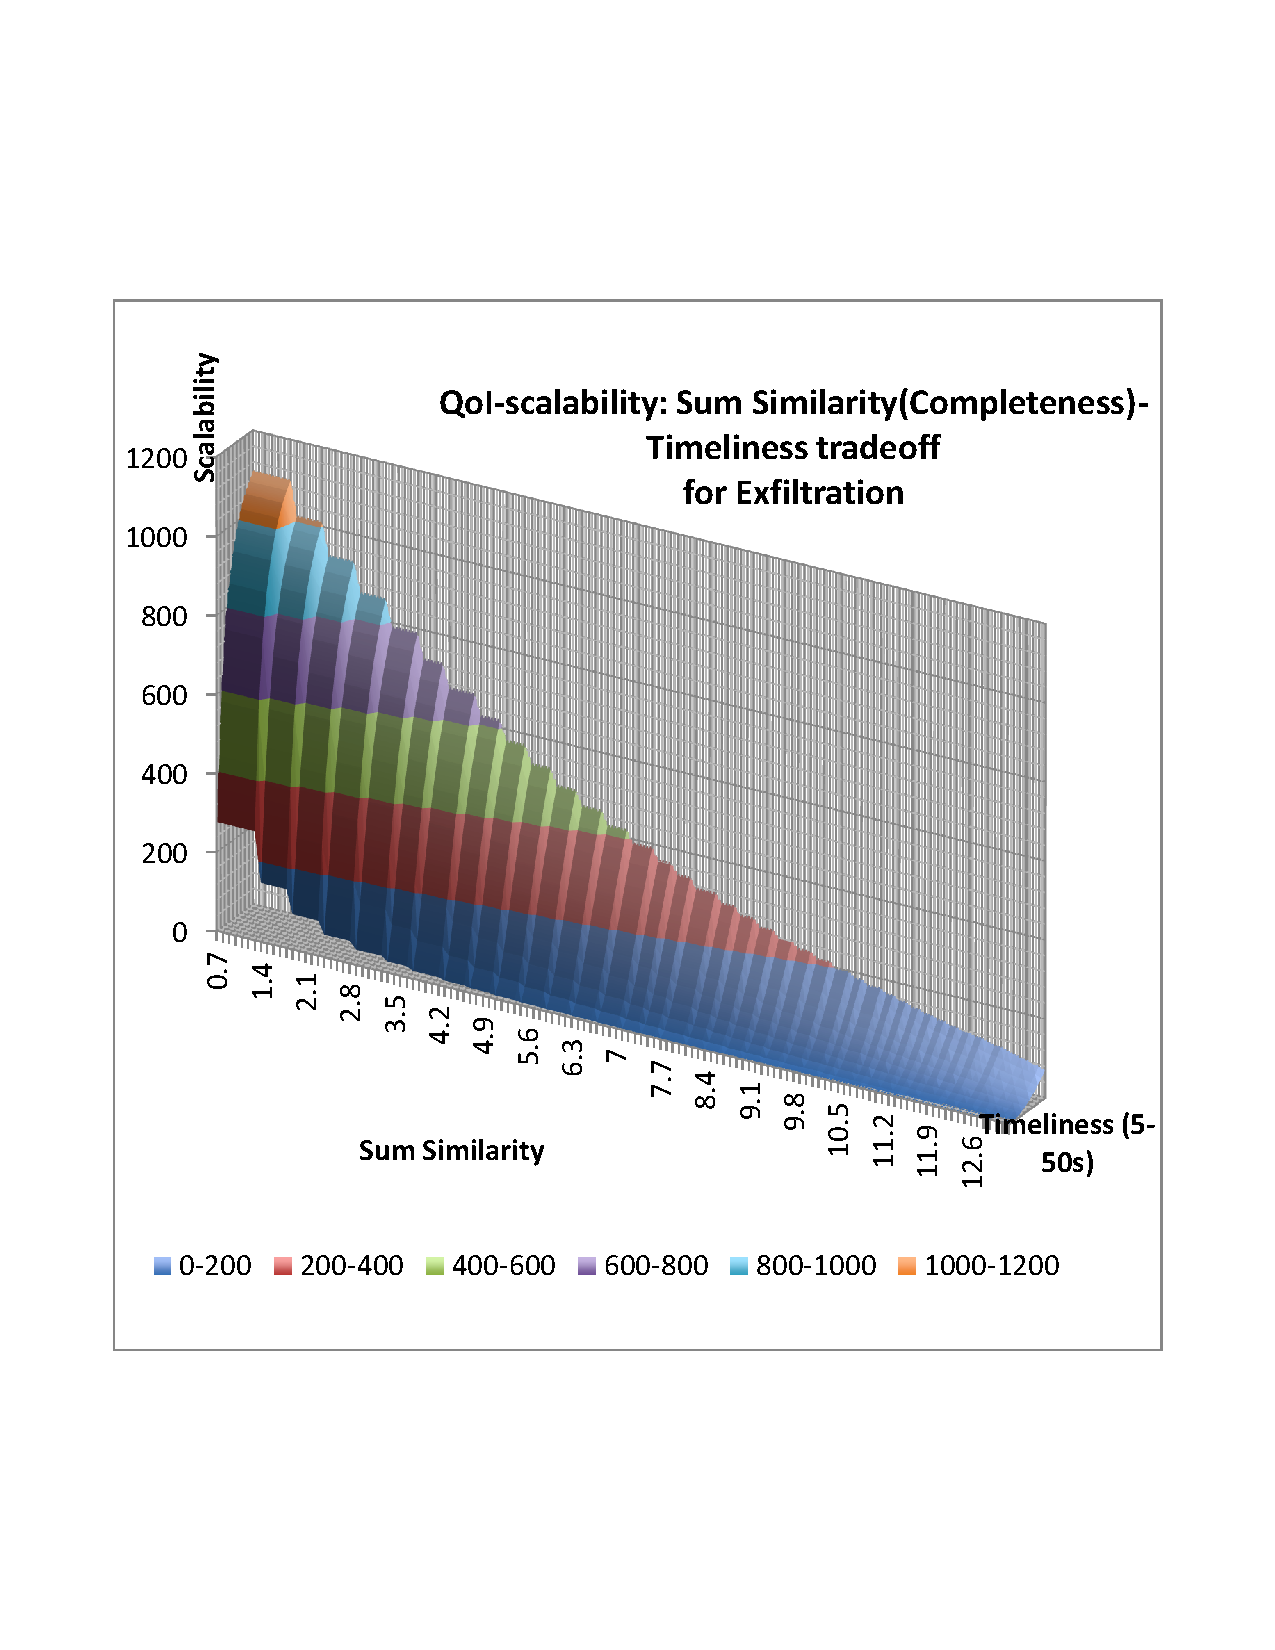
\includegraphics[scale=0.35]{figures/topk_uni.pdf}
        \label{fig:3dplot1}
        }

    \subfigure[Flooding]{
        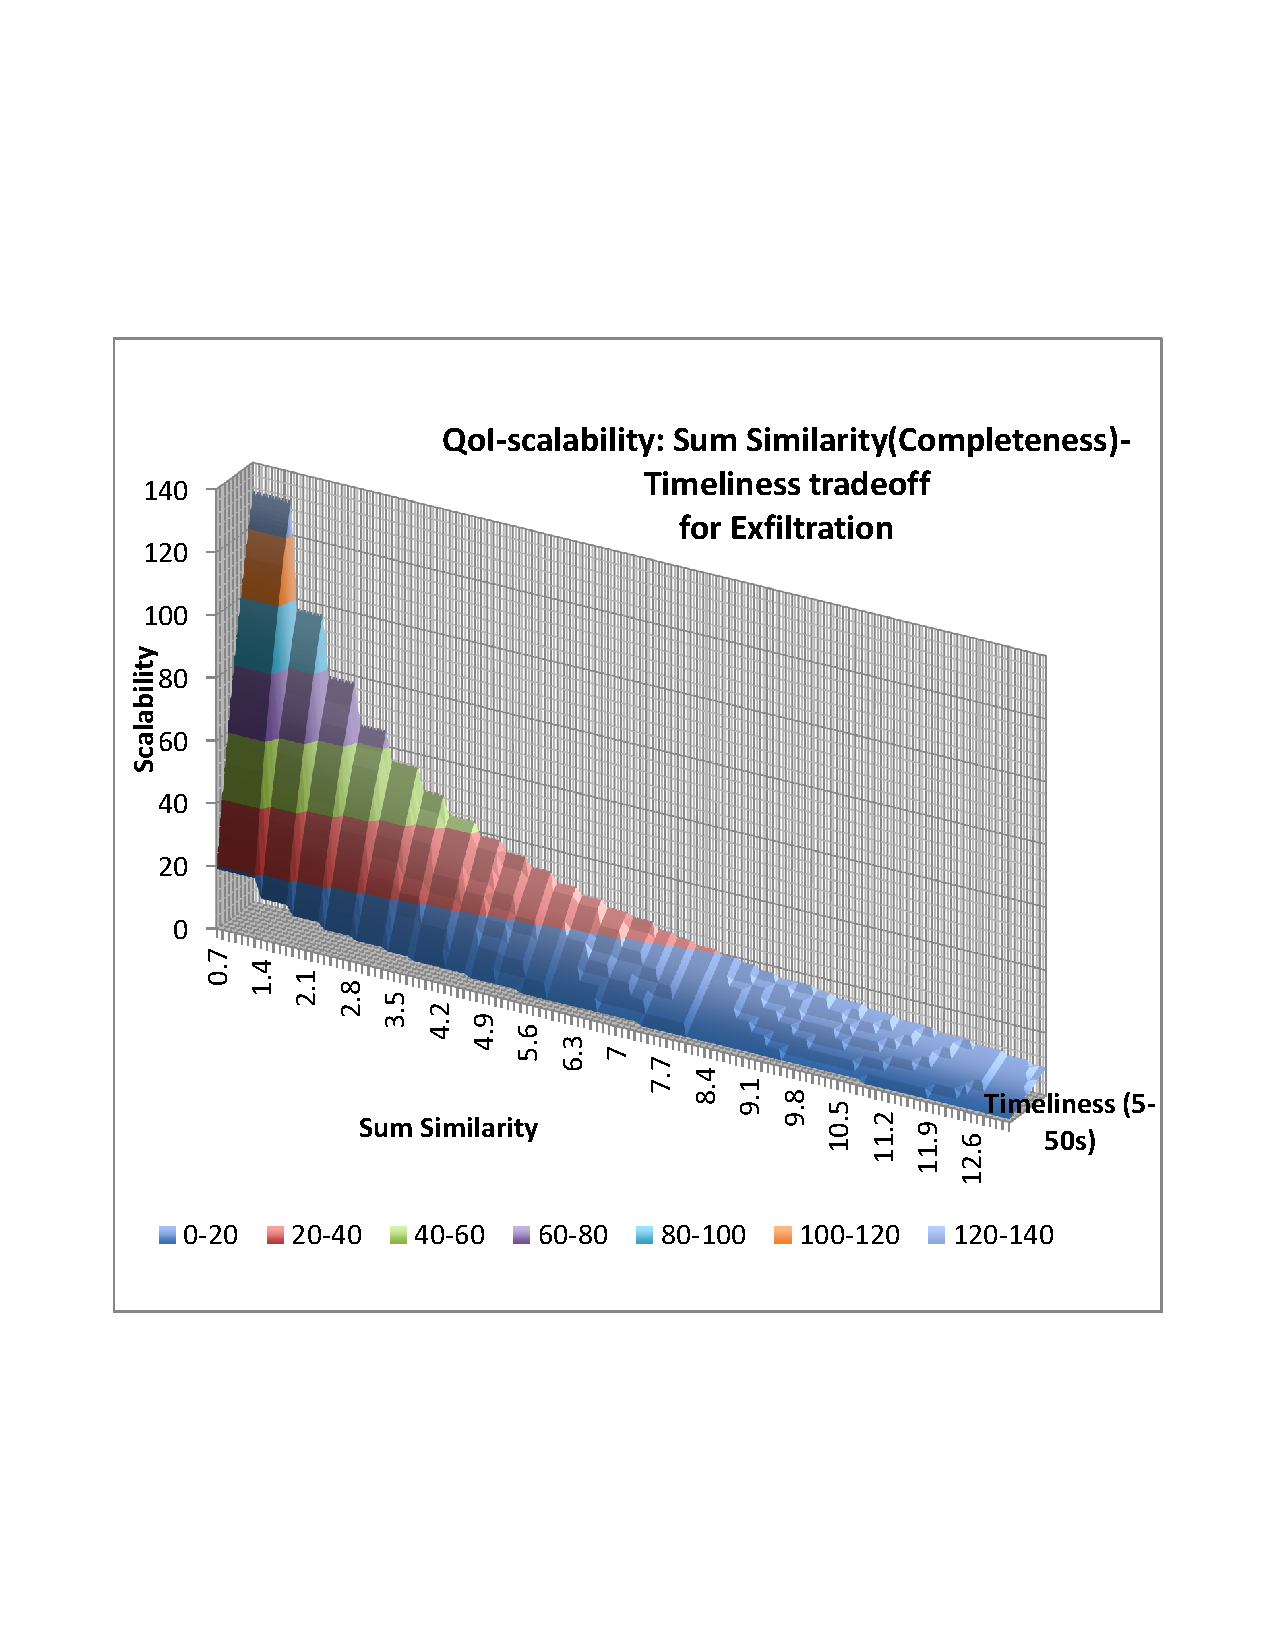
\includegraphics[scale=0.35]{figures/topk_fld.pdf}
        \label{fig:3dplot2}
        }

   \caption{Top-K:  Sum Similarity vs. Scalability vs. Timeliness}
\end{figure}


\begin{figure}
\centering
    \subfigure[Unicast Traffic]{
    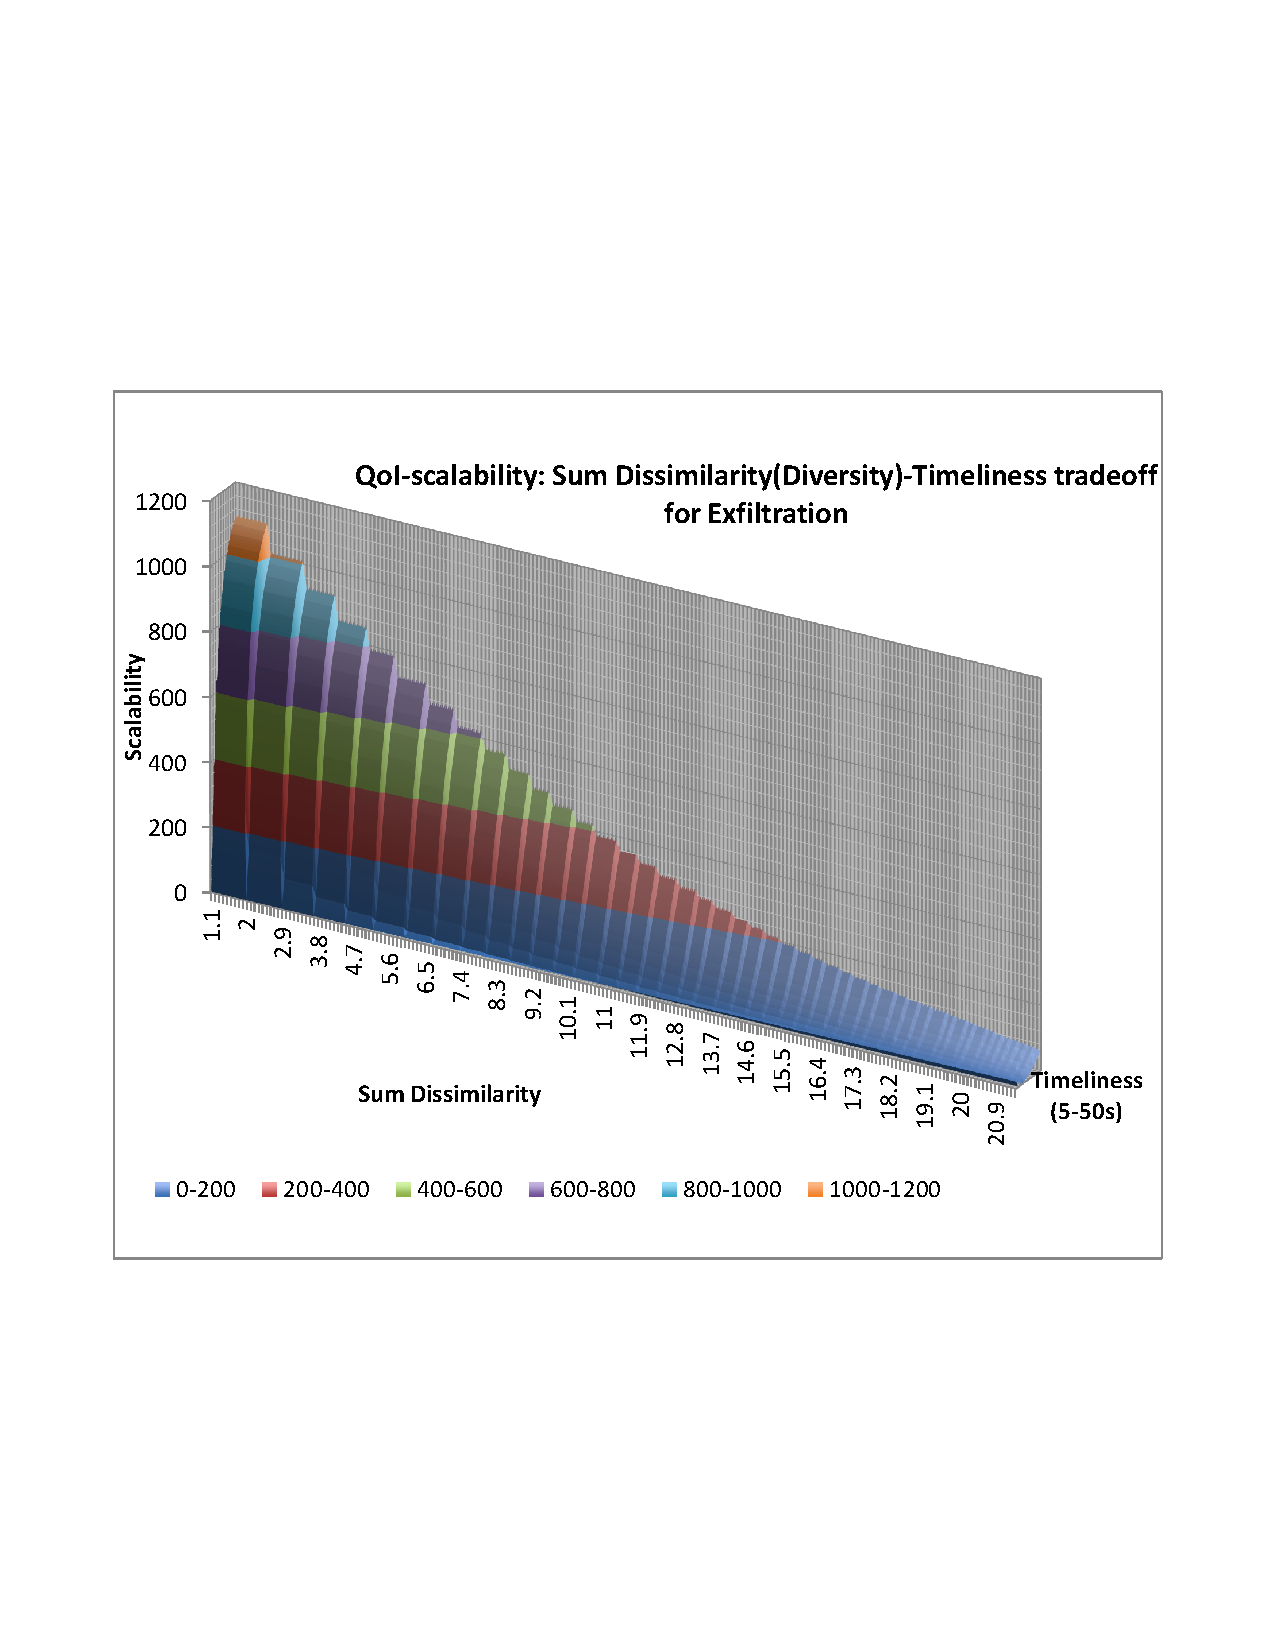
\includegraphics[scale=0.35]{figures/span_uni.pdf}
    \label{fig:3dplot3}
    }

    \subfigure[Flooding]{
    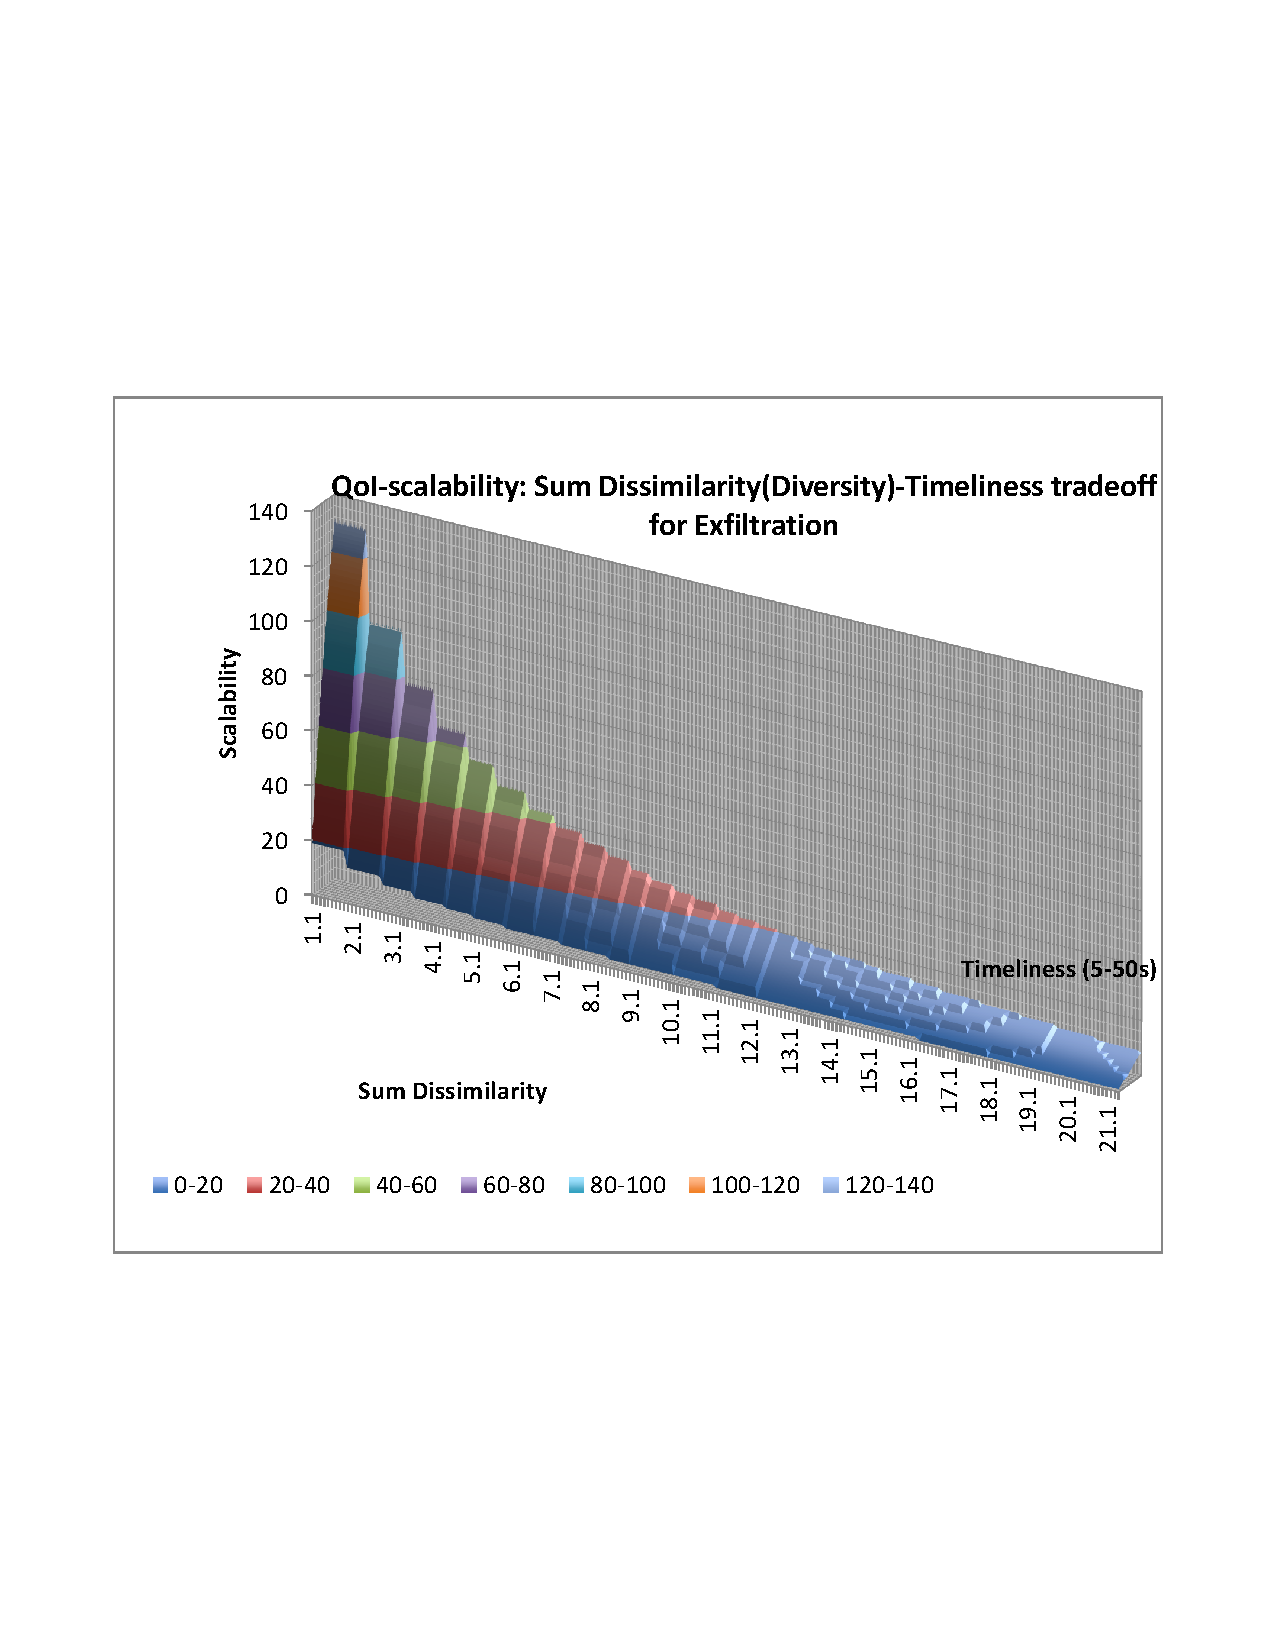
\includegraphics[scale=0.35]{figures/span_fld.pdf}
    \label{fig:3dplot4}
    }
   \caption{Spanner:  Sum Dissimilarity vs. Scalability vs. Timeliness}
\end{figure}

Clearly, there is a remarkable difference in the scalability depending upon
the QoI. %, and hence QoE desired.
The fact that QoI makes a difference is not surprising, but the {\em magnitude} of the
impact is surprising, along with the fact that there are some critical
thresholding points. Our preliminary work shows that
scalability analysis with QoI awareness has the potential to
open up new tradeoff points with
significant potential benefits in scalability. For instance, it can
potentially indicate when it makes sense to reduce QoI a bit and possibly
gain significantly in scalability (e.g. from QoI=(10,5) to QoI=(10,10) in Figure
\ref{fig:scal-log}) and when such reductions will only give a marginal
increase in scalability
(e.g. from QoI=(3,40) to QoI=(3,45) in Figure \ref{fig:3dplot1}).



\subsection{Scalably Feasible QoI Regions}
For the special case where each node possesses one image, we have observed the following dilemma. To achieve a certain level of desired QoI \text{q}, which can be defined as $(C,T)$ for Top-K queries and $(D,T)$ for spanner queries, the completeness/diversity attribute necessitates a number $K_{req}(q)$ images to be collected. When each node can contribute with at most one picture, this implies a minimum network size of $K_{req}(q)$ that is necessary for the QoI level. On the other hand, the same QoI pair also results in a maximum network size $S(q)$ from the scalability framework.
When $S(q)<K_{req}(q)$, it is not possible to provide QoI level \text{q}. Hence, we state that the QoI level \text{q} is infeasible, or \emph{scalably infeasible}.

This phenomenon defines the concept of \emph{scalably feasible QoI regions}, which define the set of QoI pairs that can be supported, given a given traffic structure. This region is given by a set of (completeness, timeliness) pairs for Top-K, and (diversity, timeliness) pairs for spanner queries. 
We demonstrate the scalably-feasible QoI regions in Figures \ref{fig:topkScalR}-\ref{fig:spanScalR}.


\begin{figure}
    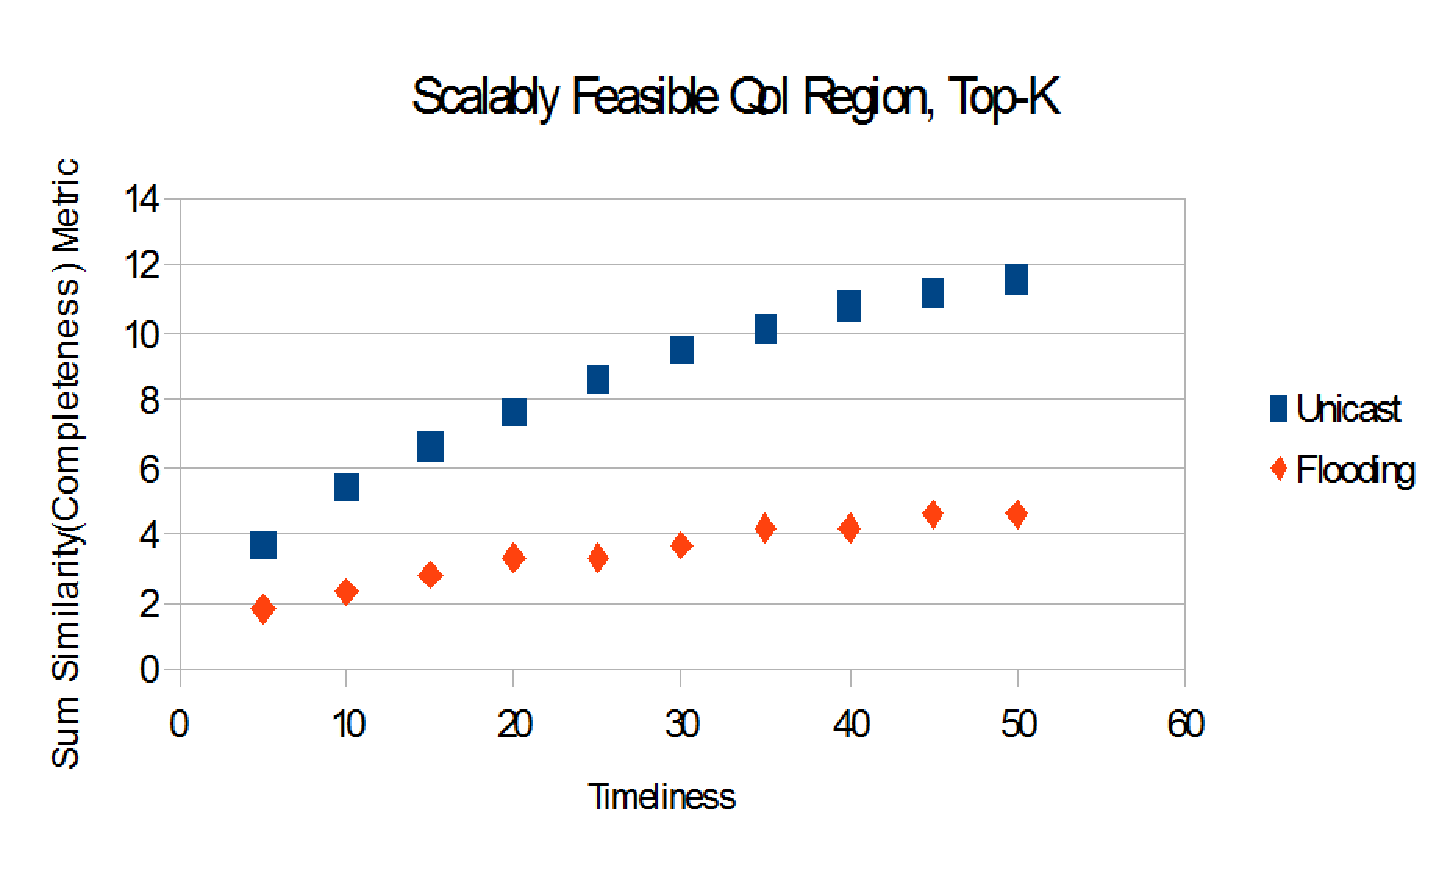
\includegraphics[scale=0.35]{figures/topkScalR.pdf}
    \caption{Feasible Scalability Region of Top-K Algorithm}
    \label{fig:topkScalR}
\end{figure}

\begin{figure}
    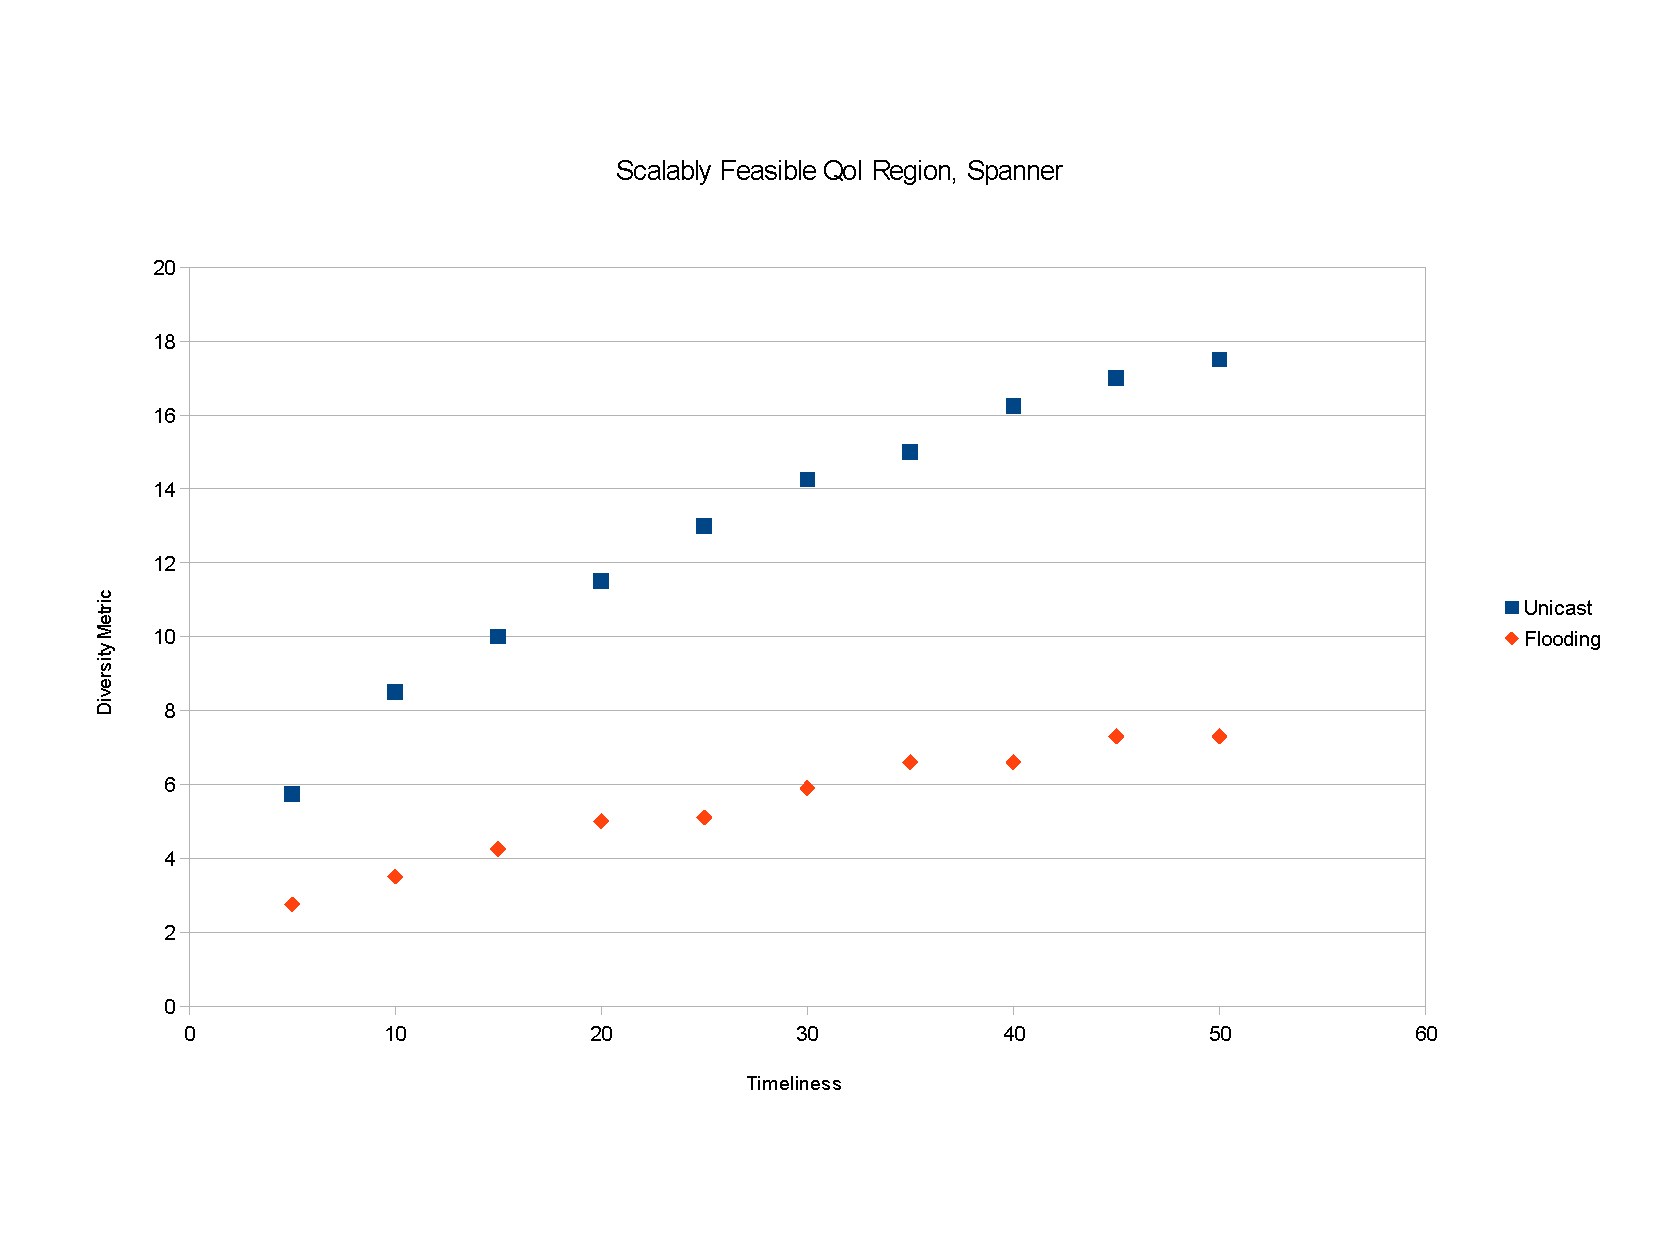
\includegraphics[scale=0.35]{figures/spanScalR.pdf}
    \caption{Feasible Scalability Region of Spanner Algorithm}
    \label{fig:spanScalR}
\end{figure}

As expected, the feasible QoI region is smaller for flooding compared with unicast. Moreover, these regions clearly demonstrate the tradeoff between the completeness/diversity that can be obtained and the timeliness that can be tolerated. 